\documentclass{subfiles}

\begin{document}
    \subsection{Entartete Störungstheorie}
        Wir betrachten das Wasserstoffatom für eine Quantenzahl $n > 1$ wegen $n^2$ facher Entartung. Wir haben zu lösen
        \[
            \frac{\braopket{n_i^{(0)}}{H_1}{n_j^{(0)}}}{E_n^{(0)} - E_{n}^{(0)}}\to\infty,
        \]
        da $E_n^{(0)} - E_{n}^{(0)} \to 0$. Zur Lösung wollen wir $H_1$ diagonalisieren und auf den Eigenraum zu dem Eigenwert $E_1$ einschränken. Dann ist 
        \[
            H|_{\text{Eig}(E_n)} = E_n\cdot I_{\deg(\text{Eig}(E_n))} + H_1|_{\text{Eig}(E_n)}.
        \]
        Ist $H_1$ diagnonalisierbar, so finden wir eine Basiswechselmatrix $U\in ?$ mit $H_1 = U^{-1}\cdot\overline H_1\cdot U$. 
        
        \subsubsection*{Beispiel: Wasserstoffatom}
            Wir betrachten das Wasserstoffatom im Hauptquantenzahlzustand $n = 2$ und der Entartung $g:= n^2 = 4$ unter Vernachlässigung des Spins. Dann sind die möglichen Eigenvektoren der Form $\ket{n,l,m}$ gerade
            \[
                \{\ket{2,0,0},\ket{2,1,0},\ket{2,1,1},\ket{2,1,-1}\}.
            \]
            Nach den Auswahlregeln $m'=m$ und $j' = j \pm 1$ fallen die Zustände $\ket{2,1,1}$ und $\ket{2,1,-1}$ weg. Wir erhalten also als einzige nicht verschwindende Kombination 
            \[
                \braopket{2,0,0}{H_1}{2,1,0} = -e\cdot E_z\cdot \braopket{2,0,0}{Q_3}{2,1,0} = -3\cdot e\cdot E_z\cdot a_B,
            \]
            wobei $a_B$ der Bohrsche Atomradius ist. 
            \begin{Aufgabe}
                \nr{} Zeige diese Gleichungskette durch Anwendung der Operatordefinitionen und einem in $z$ Richtung anliegenden elektrischen Feld $E = (0,0,E_z)$.

                \nr{} Definiere noch einmal den \emph{linearen Stark Effekt} und den \emph{quadratischen Stark Effekt}.
            \end{Aufgabe}
            \noindent Wir erhalten also die Matrixdarstellung
            \[
                H_1|_{\text{Eig}(E_2)} = \begin{pmatrix}
                    0 & -3\cdot e\cdot E_z\cdot a_B & 0 & 0 \\
                    -3\cdot e\cdot E_z\cdot a_B & 0 & 0 & 0 \\
                    0 & 0 & 0 & 0 \\
                    0 & 0 & 0 & 0
                \end{pmatrix}.
            \]
            Damit hat die Matrix $H_1|_{\text{Eig}(E_2)}$ und dessen charakteristisches Polynom $\chi_{H_1|_{\text{Eig}(E_2)}}$ die Eigenwerte $\lambda_1,\lambda_2 = 0$, $\lambda_3 = 3\cdot e\cdot E_z\cdot a_B$ und $\lambda_4 = -3\cdot e\cdot E_z\cdot a_B$. Optisch haben wir dann einen Verlauf der Form 
            \begin{figure}[H]
                \centering
                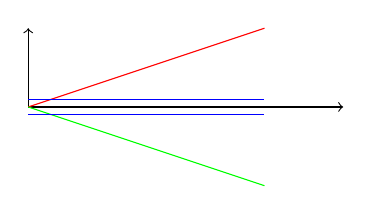
\begin{tikzpicture}
                    \draw[->] (0,0) -- (0,1);
                    \draw[->] (0,0) -- (4,0);

                    \draw[red] (0,0) -- (3,1);
                    \draw[green] (0,0) -- (3,-1);
                    \draw[blue] (0,-0.1) -- (3,-0.1);
                    \draw[blue] (0,0.1) -- (3,0.1);
                \end{tikzpicture}
            \end{figure}

    \subsection{Zeitabhängige Störungstheorie}
        Unsere störungstheoretische Betrachtung hat nun die Form $H(t) = H_0 + H_1(t)$. Unsere Fragestellung ist nun, ob sich die Wahrscheinlichkeit für einen Übergang aus dem Grundzustand mit der Zeit $t$ ändert, wenn dieser bei $t = 0$ vorgelegen hat. Hierzu benötigen wir formale Werkzeuge.
        \subsubsection*{Schrödinger-Bild}
            Für die zeitabhängige Schrödingergleichung gilt zunächst $H(t)(\psi(t)) = \cmath\cdot\hbar\cdot\dv{t}\psi(t)$ mit einem Anfangswert $\psi(0) = \psi_0\in H^2(\R)$. Durch Linearen Zusammenhang über die zeitabhängige Schrödingergleichung nehmen wir linearen Zusammenhang zwischen $\psi(t)$ und $\psi_0$ an. Damit konstruieren wir eine Transformationsfunktion $\Phi(t,t_0):H^2(\R)\to H^2(\R)$ mit $\psi(t) = \Phi(t,t_0)(\psi_0)$. Mit Normalisierungsbedingung $\dabs{\psi(t)}{} = 1$ für alle $t\in\R_{>0}$ folgern wir für die Darstellungsmatrix (Wronski Matrix) von $\Phi(t,t_0)$ mit Namen $W(t,t_0)$ eine unitäre Matrix. Damit ist $W(t,t_0)$ invertierbar und es gilt
            \[
                \cmath\hbar\codt\dv{t}\Phi(t,t_0) = H(t)\circ \Phi(t,t_0).
            \]
            Es löst dann nach Ana3 Theorie die Exponentialfunktion diese DGL, von der Form $W(t,t_0) = \exp(-\cmath\cdot (t-t_0)\text{dm}(H)/\hbar)$, wobei $\dm(H)$ die Darstellungsmatrix zu $H$ ist. 
            \begin{Aufgabe}
                \nr{} Notiere einmal nach Definition den Erwartungswert einer Observablen $T$ im Zustand $\psi(t)$. 
            \end{Aufgabe}

        \subsubsection*{Heisenberg-Bild}    
            Aus der Aufgabe kennen wir nun die Beschreibung des zeitabhängigen Erwartungswertes von $T$ in dem Zustand $t$. Diesen können wir durch die Matrizen $W(t,t_0)$ und $W(t,t_0)^{-1} = W(t_0,t)$ aufspalten zu 
            \[
                \langle T\rangle_{\psi(t_0)} = \langle\psi(t_0)|\ubra{\Phi(t_0,t)\circ T\circ \Phi(t,t_0)}{T_H(t)}|\psi(t_0)\rangle.
            \]
            Wir nennen dann $\braopket{\psi_0}{T_H(t)}{\psi_0}$ das \emph{Heisenbergbild} von $T$ zum Zeitpunkt $t$. 
            \begin{Aufgabe}
                \nr{} Berechne die zeitliche Ableitung $\dv{t}T_H(t)$ und verwende $\dv{t}\Phi(t_0,t)\circ T\circ\Phi(t,t_0) = \id_\mcH = \Phi(t_0,t)\circ T\circ \bbra{\dv{t}\Phi(t,t_0)}$. 
            \end{Aufgabe}
            Mit der Aufgabe erhalten wir dann die \emph{Heisenberggleichung}
            \[
                \dv{t}T_H(t) = \frac{\cmath}{\hbar}\cdot \Bbra{H_H(t)\circ T_H(t) - T_H(t)\circ H_H(t)} + \Phi(t_0,t)\circ\dv{\tau}T(\tau)\circ\Phi(t,t_0),
            \]
            wobei $H_H := \Phi(t_0,t)\circ H\circ\Phi(t,t_0)$. 

        \subsubsection*{Wechselwirkungs-Bild}
            Unser Ziel ist es nun, die zeitabhängige Schrödingergleichung mit Störung zu betrachten. Wir haben die Form $H = H_0 + H_1$, also $\cmath\hbar\cdot\dv{t}\psi(t) = (H_0 + H_1)(\psi(t))$ mit einem Startwert $\psi(0) = \psi^{(0)}(0) = \ket{n}$ als Eigenzustand von $H_0$. Wir verwenden dann damit den Ansatz
            \[
                \psi(t) = \exp(-\cmath\cdot t\cdot \text{dm}(H_0)/\hbar)(\psi_I(t)).
            \]
            Damit ergibt sich für $\psi_I(t)$ nach Definition die Beziehung
            \[
                \cmath\hbar\cdot\dv{t}\psi_I(t) = H_{1,I}(t)(\psi_I(t)) := \bbra{\Phi(t_0,t)\circ H_1(t)\circ\Phi(t,t_0)}(\psi_I(t)).
            \]
            Wir nennen $H_{1,I}(t)$ die \emph{Wechselwirkungs-Hamiltonfunktion}.
            \begin{Aufgabe}
                \nr{} Berechne nun die Änderung des zugehörigen Operators $T_I$. 
            \end{Aufgabe}

        \subsubsection*{Fermis goldene Regel}
            Wir wollen nun die Gleichung $\cmath\hbar\cdot\psi_I(t) = H_{1,I}(t)(\psi_I(t))$. Durch Integrationsansatz erhalten wir 
            \[
                \psi_I(t) = \psi_I(0) + \frac{1}{\cmath\hbar}\cdot\int_0^t H_{1,I}(\tau)(\psi_I(\tau))\dd\tau.
            \]
            Unter der Approximation $\psi_I(\tau)\approx \psi_I(0)$ können wir das Integral noch leicht umformen. Aus dieser Idee können wir die \emph{Fermis goldene Regel} herleiten.
            \[
                \Gamma_{i\to f} = \frac{2\pi}{\hbar}\cdot\rho_f(E_i)\cdot\braopket{f}{H_1}{i}^2,
            \]
            wobei $\rho_f(E_i)$ die \emph{Zustandsdichte} der Endzustände und $\Gamma_{i\to f}$ die \emph{Übergangsrate} von $i$ nach $f$ ist.



 
\end{document}